%a % comment anything after % until the end of the line

%minimum references to begin our article
\documentclass[12pt]{article}
\usepackage[english]{babel}
\usepackage[utf8]{inputenc}
\usepackage[T1]{fontenc}
\usepackage{graphicx}
\usepackage{fancyhdr}
\usepackage{hyperref}
\usepackage{float}
\usepackage{amsmath}
\usepackage[margin=1in]{geometry}
\usepackage{indentfirst}
\usepackage{titlesec}
\newcommand{\sectionbreak}{\clearpage}


\pagestyle{fancy}
%\cfoot{}
% the last extension makes it possible to add images

%presentation of the document
\title{Authorship Attribution\smallbreak Knowledge Aquisition project}
\author{Julien \textsc{BOUVET}, Prateek \textsc{BHATNAGAR}, \\
	Thierry \textsc{GAUGRY}, Gabriel \textsc{PREVOSTO}, \\
	Liantsoa \textsc{RASATA-MANANTENA}}
\date{03/31/2015}
\setlength\parindent{15pt}
\begin{document}

\maketitle
%\vfill %tous les vfill prennent la même place
%\begin{figure}[!h]
%\centering
%\includegraphics[width=\textwidth]{Parties/Images/Logo}
%\label{fig:logo}
%\end{figure}
%\vfill
%\vfill

\newpage
%to add a table of contents
\tableofcontents
\newpage

\section{Introduction}					\label{sec:introduction}			The objective of this report is to quickly explain both what we had to do and what we've done for our project in knowledge acquisition. 

\subsection{Authorsip Attribution}

There are two objectives for this project. The first one is to make us understand the knowledge acquisition course better, studying and implementing a software solution, to solve a classical problem of this domain.\\
The second objective is to implement a software which is able to guess the author of a given article. So it has to build a classifier given a training set, and then use it to find the author of a given article from a test set.

\subsection{Organization}

For this project we are divided in groups of 6 students, and we have 4 hours to do all the work. Because we are aware that it is quite a short time to do so, we decided to use these few hours to split the work, and discuss about the directions we were heading to. 
As a first step, we all did some documentary research and studied what is currently existing and may be helpful for the project.\\
After that we met, to chose which of these we may use, and therefore to split the work following the architecture of resulting software.

\subsection{Choice of the language}

Because of the limited time to do the project, we decided to use a language that everybody in the group knows, which makes implementation easy, and can work on several platforms. We chose Java, mainly because we all know it pretty well, which saved us a lot of time.\\
Moreover, there are a lot of libraries on this particular subject implemented in Java.

\section{The two models chosen}			\label{sec:models}				One constraint in this project is to build two different classifiers to compare their efficiency. So we choose to build one classifier based on the style of writing (punctuation, number of words per sentence ...) and one based on the content of the article (adjectives, common words...).

Here is a graphical recap of how the project is structured.
\begin{figure}[h]
	\centering
		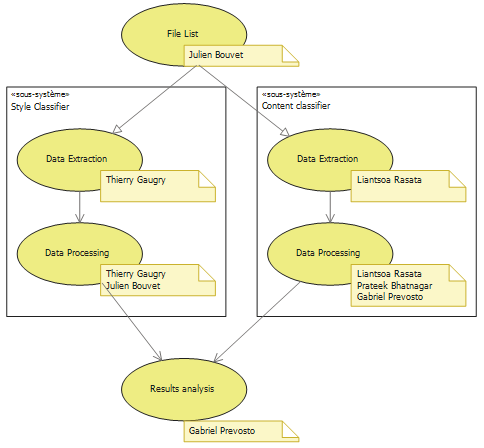
\includegraphics{Images/organization.png}
	\caption{Organization}
	\label{fig:organization}
\end{figure}

The first step is to build the list of the files, that the algorithms will need to retrieve some good information for the classifiers.\\
Then, from the files given by the previous step, we'll extract data for the first classifier (\ref{lab:data1}) and for the second (\ref{lab:data2}). This step creates a new, understanding representation of the articles, based on its classifier features.\\
After that, the style based classifier (\ref{lab:clas1}) or the content based classifier\ref{lab:clas2} will use all this data to decide who is the author of a given text.\\
To finish this, we added a results analysis (\ref{lab:ana}) step, to understand what is actually working or not, and compare the two classifiers.


\section{Stemming : why and how ?}			\label{sec:stemming}			
We do not need this this part, no need to stem for tagging.

\section{The first classifier}				\label{sec:classifier1}
\subsection{Data acquisition}				\label{sec:data1}				The parameters considered were :
The data extraction was done in java using standard libraries

\subsection{Data processing}				\label{sec:processing1}			\subsubsection{Classifier}

The classifier used was a K-nearest neighbors classifier. It is easier to implement than other classifiers, yet it gives, most of the time, pretty good results.
It was developed in java from scratch, using the standard libraries, in a single class : KNearestNeighborsClassifier. It uses two important methods : getNeighbors() and getResponse().
getNeighbors returns the list of the k nearest neighbors, with k that can be parametrized when building the classifier.
getResponse give the classifier's guess for the author of the article.

Due to the disparity of the features considered, all value have been normalized on a 0 to 1 scale.


\subsubsection{Problems}
The problem with this classifier, is that the results are not as good as we hoped. We knew the style would be harder to detect, but even on the training set the success ration is under 50\%. Knowing by heart is not the solution, so we didn't expected a 100\% success rate, but still it's a little bit deceiving. 

But, where do these poor results come from ? It's not a problem of implementation, but it come from the features. Indeed, we clearly lack of recognizable features. Moreover, some of them could be deduced from the others : The number of lines is the number of ".", "?" and "!" for example.

\section{The second classifier}				\label{sec:classifier2}
\subsection{Data acquisition}				\label{sec:data2}				\label{lab:data2}

For this second section, we decide to focus on the author's style. In fact, each writer possesses some unique characteristic which is called the authorial or writer invariant in stylometry\footnote{Application of the study of linguistic style}. This later is constant for all texts written by an author and different of other authors. The authorial invariant are based on textual properties belonging to either of four categories : lexical, syntactic, structural and content-specific.
\begin{itemize}
	\item Lexical frequencies : the total of words or characters or the average number of words per sentence.
	\item Syntactic features : the structure of sentences which can be simple, complex, conditional or built in punctuation marks. 
	\item Structural attributes : the organization of the text (drawings, headings, signatures).
	\item Content-specific properties : the recognition of some keywords which have special meaning and are importance for the text.
\end{itemize} 

\subsubsection{The second representation}
For the second representation of the data, we decide to work on Part-of-speech Tagging which is very useful in information retrieval. In our case, we want to attribute an author to an unknown text in function of the frequency of using a part-of-speech. 

\subsubsection{Part-of-speech tagging}
Part-of-speech tagging is the process of assigning a part-of-speech to each word in a sentence as noun, verb, adjective, adverb, article, preposition, pronoun, conjunction and interjection.\\

For examples:

\textbf{Heat} is a noun but also can be a verb.

\textbf{in} is a preposition but also can be a noun or an adverb.

To do POS tagging, we choose a set of tags to assign word.

Here is an example of result of the tagging: 

the/DT higher/JJR minimum/JJ wage/NN sign/NN into/IN law/NN tuesday/NNP will/MD be/VB welcome/JJ relief/NN for/IN million/CD of/IN workers/NNS ./.

\begin{itemize}
	\item DT stands for determiner.
	\item JJR stands for adjective, comparative.
    \item JJ stands for adjective.
    \item NN stands for noun.
    \item VB stands for verb base form.
    \item NNP stands for proper noun singular.
    \item NNS stands for noun plural.
    \item MD stands for modal.
    \item IN stands for preposition or subordinating or conjunction.
    \item CD stands for cardinal number.

\end{itemize}



\subsection{Data processing}				\label{sec:processing2}			\label{lab:clas2}

\section{Comparison of the two classifiers}		\label{sec:comparison}
\subsection{The result evaluation methodology}	\label{sec:evaluation}			In this part, we will refer to the following : 
\begin{itemize}
	\item \emph{TP} : Number of positives predicted as such
	\item \emph{TN} : Number of negatives predicted as such
	\item \emph{FP} : Number of positives predicted as negatives
	\item \emph{FN} : Number of negatives predicted as positives
\end{itemize}
They are also illustrated in figure \ref{fig:prec_rec}.

At the end of our calculus, we generate the confusion matrix.
This matrix indicates, for any given square (i,j), how many items of the class i were predicted of class j.
An example of a confusion matrix for a binary prediction is given in figure \ref{fig:confusion}.

\begin{figure}[!h]
\centering
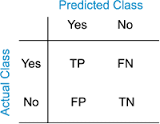
\includegraphics[width=.3\textwidth]{Images/confusion.png}
\caption{An example of a confusion matrix.}
\label{fig:confusion}
\end{figure}


In order to test the performance of our classifiers, we rely on a few indicators, processed from the confusion matrix :
\begin{itemize}
	\item \emph{Precision} indicates how many of the selected items are relevant
		\begin{equation*}
		Precision = \frac{TP}{TP+FP}
		\end{equation*}
	\item \emph{Recall} indicates how many relevant items were selected 
		\begin{equation*}
		Recall = \frac{TP}{TP+FN}
		\end{equation*}
	\item The \emph{F-Measure} takes into account both of those values
		\begin{equation*}
		F\-Measure = \frac{2\times Precision\times Recall}{Precision + Recall}
		\end{equation*}
\end{itemize}
These values are illustrated in figure \ref{fig:prec_rec}.

\begin{figure}[!h]
\centering
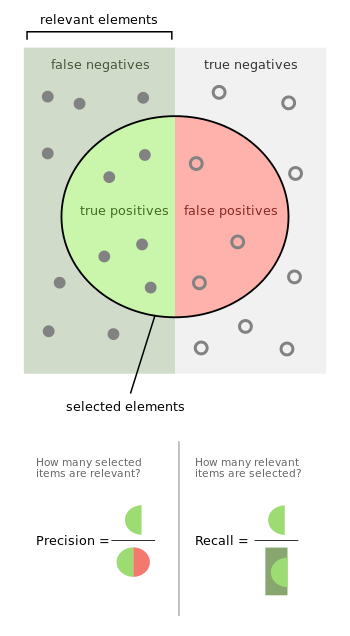
\includegraphics[width=.5\textwidth]{Images/prec_rec.png}
\caption{Precision and recall.}
\label{fig:prec_rec}
\end{figure}


For muticlass classifiers, Precision and Recall are an average of the precision and recall of the binary classifiers for each class.
\begin{equation*}
Precision_{Multiclass} = \frac{\sum_{i=0}^{n} Precision(i)}{n} 
\end{equation*}
\begin{equation*}
Recall_{Multiclass} = \frac{\sum_{i=0}^{n} Recall(i)}{n} 
\end{equation*}

\subsection{The final verdict}				\label{sec:verdict}				In the end, we processed te results of our calculus, in order to compare them.

\subsubsection {Results for the first classifier}

The first classifier's results were quite poor, with low precision and recall (approx. 0.15 each).
Tests on other data has proven our classifier to work (we tested it with simple examples, like flower categorization).
The reasons why it worked so poorly on authorship attributions are because the information we chose to extract was not sufficient to produce accurate results.


\subsubsection {Results for the second classifier}

The results for the second classifier, unlike those of the first classifier, were satisfactory, with a slight issue : the analysis using part-of-speech tagging used too much RAM to be run on the entire database.
We decided to run it on a subset of the available authors, and it gave good results (Precision of 0.53, Recall of 0.50, F-Measure of 0.51).
That basically means that half of the texts are predicted correctly, which is not bad considering the test was performed with 11 authors.
It is a lot better than randomness, which would only have guessed correctly 1/11 times.


\subsubsection {Conclusion}

We tried two classifiers and only one gave us good results. Classifying with the length of sentences, frequency of punctuation, etc. did not prove sufficient, but  part-of-speech tagging proved to be more reliable.

\section{Conclusion}					\label{sec:concluision}			\input{"Text/conclusion.tex"}

\end{document}
